% ------------------------------------------------------------------
% Exemplo de introdução gerada por textos dummys a partir do
% lipsum
%-------------------------------------------------------------------


\chapter{Introdução}
\label{cap:intro} % faço a referência na bibliografia
\section{Motivação e Estado da Literatura}

O modelo descrito em \citeonline{breiman2001random} apresenta um procedimento de estimação de uma sequência de Árvores de Decisão a partir de subamostras independentes e identicamente distribuídas de um conjunto de dados. O nome da técnica vem do algorítimo consistir em montar uma coleção de Árvores de Decisão e empregar procedimentos de amostragem para que cada árvore individual seja exposta a uma subamostra aleatoriamente encontrada dos dados.

Modelos de Floresta Aleatória (no original, \texit{Random Forest}) têm aplicações em áreas variadas. Pesquisa biomédica, identificação de padrões em visão computacional, finanças e microeconomia aplicada são áreas que já difundiram seu uso. Um entendimento próprio de efeitos marginais é particularmente importante na aplicação econométrica da técnica porque permite a eventual construção de regressão em dois estágios e formas mais precisas de estimar parâmetros em desenhos de Variáveis Instrumentais.

Em revisões de literatura \cite{siroky2009navigating, biau2016random} costuma-se enfatizar alguns resultados sobre a performance da técnica - que entrega capacidade preditiva elevada \cite{gu2018empirical}. Geralmente falando, com o crescimento do número de árvores o primeiro momento da distribuição do erro de previsão fora da amostra converge a zero, seu segundo momento diminui e o custo computacional de efetivamente estimar a floresta cresce com derivada decrescente. O procedimento de estimação original de Breiman fornece um estimador (i) não-viesado, (ii) consistente e (iii) factível, todas propriedades centrais na aplicabilidade dessa técnica. Assim como em modelos lineares, também é possível decompor variância explicada do modelo. \citeonline{stijven2011separating} introduziram algumas ferramentas de regressão simbólica no modelo original de Breiman para explicar importância relativa de regressores e há maneiras de abordar o mesmo problema usando Valores de Shapley, vindos da Teoria dos Jogos Cooperativos \cite{cohen2007feature}.

Avanços recentes na literatura focam em frentes diversas. Uma que dialoga com o problema a ser estudado nesta monografia é como conciliar os modelos com bancos de dados com uma quantidade crescente de variáveis e, portanto, alta dimensionalidade. Uma direção de pesquisa foca em adequar a teoria que fundamenta a técnica ao contexto em alta dimensão \cite{athey2019generalized}, outra em seleção de variáveis e redução de dimensionalidade \cite{hastie2015statistical}. 

Esse esforço de pesquisa gerou um princípio de entendimento melhor de efeitos de tratamento. \citeonline{ikonen2016machine} desenvolveu uma tećnica (rudimentar) de estimação de efeitos de tratamento sintéticos - uma extensão da técnica de Controles Sintéticos \cite{abadie2010synthetic}. A dupla Athey e Wager, particularmente ativa neste debate, deixou algumas contribuições importantes. Notadamente em contexto de alta dimensão \cite{athey2018approximate} e em contexto de tratamentos heterogêneos \cite{wager2018estimation}. 

Em modelos lineares paramétricos sabemos ser possível aproximar não-linearidades arbitrárias imputando no modelo funções não-lineares dos regressores originais, afinal o que caracteriza um modelo estatístico univariado como \textbf{linear} é ter derivadas constantes em relação aos parâmetros, não nos regressores. Em Florestas Aleatórias sabemos que por desenho não é necessário inserir funções não-lineares dos regressores para acomodar não-linearidades, então essa ponte já está estabelecida, no entanto pouco é sabido sobre o comportamento dos efeitos marginais.

O objetivo desta monografia é propor um procedimento sistemático de estimação de efeitos marginais de tratamento, avaliar o quão (in)constantes são os efeitos marginais e o quão sensíveis aos outros regressores eles são. A metodologia empregada será estimar um modelo de Floresta Aleatória, computar suas previsões na observação mediana dos dados e em observações medianas com perturbações controladas em cada regressor. O resultado é uma curva relacionando valor predito com valores dos regressores, cuja derivada - se computável - entrega os efeitos marginais.

\section{Teoria Preeliminar}

A unidade mais simples de uma Floresta Aleatória é uma Árvore de Decisão \cite{breiman2017classification} então a exposição daí partirá. Vamos construir uma árvore de decisão.

Uma \textbf{observação} de $k$ variáveis é um vetor $x \in \R^k$, em que cada dimensão representa uma variável diferente. Variáveis binárias podem ser representadas por pares $0$ e $1$. Definimos o \textbf{Espaço de Mensuração} $\mathbf{X}$ como sendo o conjunto de todos os vetores $x$ possíveis para os suportes definidos. Por exemplo: se uma dimensão deste espaço representa idade, entendemos que seu suporte está nos inteiros positivos entre $0$ e, digamos, $120$. Se uma variável é uma categoria binária, então seu suporte está em $0$ e $1$. 

As observações podem ser entendidas como pertencendo a \textbf{classes} (como por exemplo, bicicletas de corrida, bicletas de passeio, bicicletas dobráveis, etc), estando a cargo do modelador definir exatamente quais classes são essas. Dizemos que o problema é de \textbf{Classificação} quando nossas observações tem suas classes em um conjunto discreto e que o problema é de \textbf{Regressão} quando há um conjunto infinito de classes disponíveis (e.g. quando a variável modelada é um preço, ou outra grandeza contínua). Classificar um paciente como sendo portador de uma doença ou não é claramente um problema de classificação. Estimar o preço de um imóvel com base em suas características é um problema de regressão. Suponha que temos um conjunto de classes $\C = \{1,2,...,J\}$ com $J$ classes. Notaremos $\C(x)$ como a classe da observação $x$. Nesta monografia a cardinalidade de $\C(x)$ sempre é unitária, trabalharemos com contextos em que não há sobreposição de classes. 

\begin{defi}
Um \textbf{Banco} é uma par de um espaço de mensuração com um conjunto de classes possíveis $(\mathbf{X}, \C})$ tal que $\forall x \in \mathbf{X} \to \C(x) \in \C$. Ademais, se temos $X \subset \mathbf{X}$ então o par $(X, \C)$ que satisfaça $x \in X \to \C(x) \in \C$ é dito uma \textbf{instância} do banco $(\mathbf{X}, \C})$.
\end{defi}

\begin{defi} Seja $(\mathbf{X}, \C)$ um Banco. Um \textbf{Classificador} é uma função $\math{C} : \mathbf{X} \to \C$.
\end{defi}

Podemos entender um Classificador de outra maneira. Defina o conjunto $A_i = \{ x \in X \,\, ; \,\, \C(x) = i\}$. Então a união $\bigcup_{i = 1}^J A_i$ é o próprio conjunto $X$ e cada $A_i$ é disjunto de todos os outros $A_{j \neq i}$.

\begin{defi}
Um \textbf{Classificador} é uma partição disjunta de $\mathbf{X}$.
\end{defi}

Estimar uma Floresta Aleatória (ou Árvore de Decisão, modelo de regressão linear, o que quer que seja) é fundamentalmente escolher entre as inúmeras possibilidades de Classificadores o mais apropriado para os \textbf{dados}. Os procedimentos estatísticos que empregamos para encontrar alguma aproximação desde "classificador ideal" são aplicados em algum tipo de amostra, convenientemente representada a partir de agora por uma instância de um Banco.

Por fim, precisamos entender a estrutura dos dados. Dizemos que se toda observação assume um vetor no $\R^k$ então dizemos que os dados têm estrutura \textbf{padronizados} ou \textbf{\textit{tidy}} \cite{tidyr}. Esta monografia se limita ao contexto de dados \textit{tidy}, como boa parte da literatura econométrica.

\section{Construindo uma Árvore de Decisão}

Antes de propriamente construir uma Árvore de Decisão, precisamos definir formalmente uma árvore em um contexto de teoria dos grafos. 

\begin{defi}
Um \textbf{grafo} é um par $G = (V, E)$, onde $V$ é um conjunto de elementos que chamamos de \textbf{vértices} e os de $E$, \textbf{arestas}. Se uma aresta conecta dois vértices, dizemos que é aresta incidente aos vértices. Notamos o conjunto de vértices incidentes a uma aresta $h$ pela função $\phi(h)$.
\end{defi}

\begin{defi}
Um \textbf{passeio} é qualquer sequência de arestas $(h_1, h_2, ..., h_{n-1})$ para os quais há uma sequência de vértices $(v_1, v_2, ..., v_n)$ de forma que $\phi(h_i) = \{v_i, v_{i+1}\}$. Uma \textbf{trilha} é um passeio em que toda aresta é distinta. Um \textbf{caminho} é uma trilha em que todo vértice é distinto. Um \textbf{ciclo} é qualquer trilha que comece e termine no mesmo vértice. Um grafo que não admite ciclos é dito \textbf{acíclico}
\end{defi}

\begin{defi}
Um grafo $G$ é dito \textbf{conexo} se para qualquer par de vértices $x, y \in V \subset G$ há pelo menos um caminho cujo vértice inicial é $x$ e o terminal é $y$. Um subconjunto de vértices de um grafo desconexo em que vale esta propriedade é dito um \textbf{componente}.
\end{defi}


\begin{defi}
Seja $G$ um grafo conexo. Se a remoção de qualquer aresta $h$ gera $G / \{h\}$ que não é conexo, então $G$ é dito uma \textbf{árvore}. Um conjunto de árvores disjuntas é dito uma \textbf{floresta}.
\end{defi}

\begin{teo}
$G$ é uma árvore se, e somente se, é conexo e acíclico.
\end{teo}

\begin{prova}
Seja $G$ um grafo conexo e acíclico e a aresta $h_1$ incidente aos vértices $x$ e $y$. Suponha por absurdo que $G / \{h_1\}$ seja conexo. Então existe alguma aresta $h_2$ incidente a $x$ e a outro vértice $z$ ao qual $h_1$ não era incidente. Como $G$ é conexo, necessariamente há um caminho que começa em $y$ e termina em $z$. Então havia, antes da remoção de $h_1$, um ciclo começando e terminando em $y$, formado pela união do caminho que liga $z$ e $y$ com $h_1$, em contradição com $G$ ser acíclico.

Suponha agora que $G$ seja conexo e que $G / h_1$ seja um grafo desconexo. Tome três vértices, $x, y \,\text{e}\, z$. Suponha sem perda de generalidade que $x$ e $y$ são ligados por $h_1$. Como $G$ é conexo há pelo menos um caminho ligando cada um destes vértices aos outros. Se $x$ tinha todo caminho indo para $z$ passando por $y$, então nenhum ciclo por incluir $x$. Se $x$ tinha um caminho para $z$ que não passava por $y$, isso contradiz $G / h_1$ ser um grafo desconexo, então de fato não há como um ciclo passar por $x$. $G$ é acíclico. \blacksquare


\end{prova}

Um classificador Árvore de Decisão é qualquer classificador que admita uma representação como Árvore. Podemos entender isso associando a cada vértice de uma árvore uma divisão dos dados. Cada divisão $D_i$ carrega duas informações: (i) um teste lógico factível para todas as observações passarem ou não (e.g. ao classificar a classe de um navio militar, nenhum com mais de $100m$ de comprimento pode ser um destróier) e (ii) uma posição na árvore, determinando quais divisões/vértices estão acima e quais estão abaixo.

\begin{figure}
    \centering
    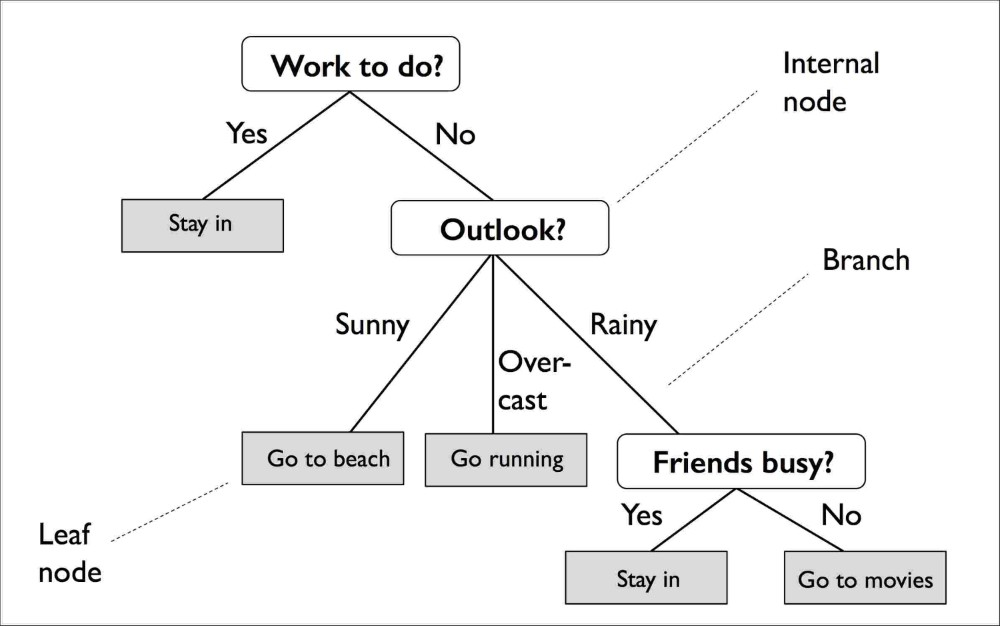
\includegraphics[scale = .25]{imagens/arvore.png}
    \caption{Um exemplo de árvore de decisão}
    \label{fig:arvore}
\end{figure}

Cada divisão quebra todas as observações que chegaram nela em exatamente dois grupos. Então toda divisão posterior gera apenas subconjuntos. Uma divisão pode ser de dois tipos: terminal e não-terminal. Se uma divisão implica classificação perfeita (todas as observações que atendem ao critério são da mesma classe), então não há por que continuar a dividir os dados e esta divisão termina seu "galho" da árvore. 


\section{Noções de Estimação de uma Árvore de Decisão}

Como podemos traduzir uma amostra $A$ em uma árvore de decisão $\A$? Um dos procedimentos mais consagrados, apresentado na primeira edição de \citeonline{breiman2017classification} será apresentado.

Primeiro definimos a \textbf{Proporção} de um vértice como um vetor contendo a proporção de cada classe observada nos dados que chegaram ao vértice. Depois, a \textbf{Impureza} do nodo. A função $\I(\cdot)$ mapeia um nodo em um número positivo limitado superiormente por um real $I$ de forma que a impureza de um nodo cuja proporção seja igual para todas as classes seja $0$ e a impureza de um nodo cuja proporção seja unitária para alguma classe seja $I$. Precisamos impor apenas que $\I(\cdot)$ seja monotonamente crescente em relação à probabilidade de cada classe. O valor específico da impureza não é relevante, desde que aumente monotonamente em relação à heterogeneidade de proporções observadas.

Tome uma divisão $D_i$ qualquer. Ela rende duas subamostras/divisões que podem ou não serem terminais, $D_{iA}$ e $D_{iB}$. Defina $P_A (D_i)$ como a proporção de casos que chegam em $D_i$ e vão para $D_{iA}$ e o mesmo para $P_B (D_i)$.

\begin{defi}
A \textbf{Qualidade} da divisão é dada pela variação na impureza: $\mathcal{Q} (D_i) := \I(D_i) - P_A(D_i) \I (D_{iA}) - P_B(D_i) \I (D_{iB})$.
\end{defi}

Note que a qualidade é uma variável aleatória. O processo de formar uma árvore de decisão a partir de um certo conjunto de dados é chamado de treinar a árvore. Escolher a divisão adequada envolve muitos recursos computacionais e selecionar a divisão que maximize a qualidade dentre as potenciais. Qualquer regra computável pode ser usada: um valor ser maior ou menor que um certo patamar, estar em uma certa faixa, etc. Os aspectos algorítmicos deste problema são interessantes porém fogem ao escopo desta monografia, discussões podem ser encontradas em \citeonline{de1991distance}.
 
 \section{Construindo uma Floresta Aleatória}
 
 A agregação das predições de árvores construídas a partir de pedaços diferentes da amostra é um passo seguinte e natural à modelagem anteriormente apresentada. Como os procedimentos de escolha de divisões são estocásticos, árvores individuais de decisão podem apresentar vieses ou baixa performance ao acaso. Se um número grande de árvores é agregado e não há relação sistemática do erro de predição com alguma variável preditiva, então os erros devem se anular com o aumento do número de árvores.
 
 \begin{defi}
 Seja $A$ uma instância de um Banco $(\mathbf{X}, \C)$. Existe um conjunto de subamostras únicas dessa instância, $B = \{ B_1, B_2, ..., B_k\}$  independentes. Seja $m(\cdot)$ a função moda. Treine em cada elemento de $B$ uma árvore de decisão $\A_i$ e chame de $F(x)$ o conjunto de imagens obtidas ao aplicar cada $\A_i$ a uma observação $x$ da instância $A$. Uma \textbf{Floresta Aleatória} é um classificador $\F : m(F(x)) \to \C$. 
  \end{defi}
  
  \begin{defi}
  Seja $A$ uma instância de um Banco $(\mathbf{X}, \C)$ com $n$ observações. Seja $F$ um conjunto de $k$ árvores de decisão treinadas em $A$ de acordo com a definição anterior. Seja $x_i$ a $i$-ésima observação da instância $A$ e, por fim, $\1(\cdot)$ a função indicadora. A \textbf{Margem} da floresta aleatória $\F$ formada pelas árvores de decisão $\A_j$ na observação $x_i$ é a função $M(\F, x_i) := \sum_{j=1}^k \1 ( \A_j (x_i) = \C(x_i) ) - \sum_{j=1}^k \1  ( \A_j (x_i) \neq \C(x_i) )$.
  
  \end{defi}
  
  
  \begin{defi}
 Para uma observação $x$ de uma instância $A$, o \textbf{Erro de Generalização} $G(\F, x) := \Prob (M(\F, A, x)) < 0)$.  \end{defi}
  
  A margem provê uma medida do quão precisa é a floresta em votar corretamente na classe verdadeira da observação. Uma margem maior sinaliza uma maior capacidade da floresta de discriminar o dado observado entre possíveis classes.  

 \begin{teo}[Convergência do Erro de Generalização] Seja $A$ uma instância de um Banco $(\mathbf{X}, \C)$. Defina a sequência $E_k = \{ G(\F_k, A, x) \}$ de forma que $\F_k = \F_{k-1} \bigcup \A_k $,  Tome as classes possíveis $\C = \{1,2,3,...,c,...,J \}$ e uma observação $x$, tal que $\C(x) = c$. Então $E_k \to \sum_{i=1}^k \1 ( \A_i (x) = c ) - \underset{}{\text{Max}} \sum_{i=1}^k \1  ( \A_i (x) \neq c) $
 
 \end{teo}
 
 \begin{prova}
 Ver o Apêndice 1 de \cite{breiman2001random}. \blacksquare
 \end{prova}
 
 \section{Organização da Monografia}
 
 Vimos como uma árvore de decisão pode distinguir observações e captar não-linearidades no processo gerador. Depois, que agregar árvores pode produzir uma espécie de mitigação de viés que uma árvore individual possa ter, construímos uma maneira de medir o quão bem o processo de voto democrático de cada árvore da floresta discrimina observações com sua Margem e que a partir dela podemos computar uma medida da performance preditiva em dados que não foram apresentados ao modelo em sua fase de treinamento. Por fim, vimos que o erro de generalização com dados desconhecidos tem um limite superior dado um tamanho de floresta. Estes são os fatos básicos do funcionamento do modelo.
 
 O capítulo 2 apresenta o algorítimo de computação dos efeitos marginais e o desenho da simulação. O capítulo 3 apresenta algumas estatísticas descritivas dos dados e das estimativas de Florestas. O capítulo 4 mostra as simulações e a computação dos efeitos marginais em si. O capítulo 5 conclui com alguns fatos estilizados.


